\chapter{Cross Correlations}\label{part: cross correlations}

Cross correlation is powerful (and very simple) statistical tool for computing the degree to which two signals are correlated (or similar). and also for computing lags.  

\section{Normalised Spatial Cross Correlation in 1d}

In signal processing, cross-correlation is a measure of similarity of two series as a function of the displacement of one relative to the other. As we all know, signal could be continuous and discrete. In this project, we only focus discrete signal. 

For discrete functions f and g, the cross-correlation is defined as:

\begin{equation*}
r=\frac{1}{N}
\sum_{i=1}^{i=N}(f(i)-\bar{f})(g(i)-\bar{g})
\end{equation*}

The problem at the moment is that the value of r is somewhat arbitrary because of the varient amplitude of signal. One way around this is to normalise signal with the root-mean-quare. Normalized cross correlation is typically done by subtracting the mean and dividing by the standard deviation. As:

\begin{equation*}
r=\frac{1}{N}
\sum_{i=1}^{i=N}
\frac{(f(i)-\bar{f})(g(i)-\bar{g})}{\sigma _{f}\sigma _{g}}
\end{equation*}

where

\begin{equation*}
{\sigma _{f}}=
\sqrt{\frac{1}{N}\sum_{i=1}^{i=N}(f(i)-\bar{f})^{2}}
\hspace{4em}
{\sigma _{g}}=
\sqrt{\frac{1}{N}\sum_{i=1}^{i=N}(g(i)-\bar{g})^{2}}
\end{equation*}

Matlab code of normalized 1d cross correlation is in appendix.


\section{Signal Offset}

If there are two signals(denote by vector) come from the same source and are just offset by some time. We can easily use cross correlation find the offset time and distance between two sensors. Just find the max value's posision of the cross correlation vector compute from two signal. Then find corresponding positions in the signal and compute the offset of the signal vector. If we know the rate and propagation speed, we can compute offset time and distance between the two sensors as follow:

\begin{equation*}
\text{offset time}=\frac{\text{offset}}{\text{sample rate}} 
\end{equation*}

\begin{equation*}
\text{distance}=\text{offset time} * \text{propagation speed}
\end{equation*}

\section{Normalised Spatial Cross Correlation in 2d}

The cros correlation can be extended to two-dimensional matrix. Condiser two matrices, t (template) and A (search region), The matrix A willl always larger than the matrix t. We can use two nested for-loops to ``leg'' t over A, compute for each ``lag'' the cross-correlation. Normolized cross correlation of two matrices defines as:

\begin{equation*}
R(lag_{x},lag_{y})=
\frac{\sum_{x,y}[A(x,y)-\overline{A_{lag_{x},lag_{y}}})][t(x-lag_{x},y-lag_{y})-\bar{t}]}
{\{\sum_{x,y}[A(x,y)-\overline{A_{lag_{x},lag_{y}}})]^2
	\sum_{x,y}[t(x-lag_{x},y-lag_{y})-\bar{t}]^2
	\}^{0.5}}
\end{equation*}

Where $\bar{t}$ is the mean of t, $\overline{A_{lag_{x},lag_{y}}}$ is the mean of A in the region under t. 

Matlab code of normalized 2d cross correlation is in appendix.

\section{Image Alignment}

Images are just a matrix of pixel values in most image processing. It is naturally think of computing cross correlation between two images to get more relation informations of them. In this task, we get two images, one of them is a section of the other. We can easily find where the section of the image fits in the whole through cross-correlation.

Here, we have a section (rocket man) show in Figure \ref{fig:rocketman} and a search region (maze) as Figure \ref{fig:maze-a}.

\begin{figure}[h!]
	\begin{center}
		\includegraphics[width=0.40\linewidth]{figures/part1/wallypuzzle_rocketman.png}
	\end{center}
	\caption{Rocket Man (section)}
	\label{fig:rocketman}
\end{figure} 

\begin{figure}[h!]
	\centering
	\includegraphics[width=0.60\linewidth]{figures/part1/wallypuzzle.png}
	\centering
	\caption{Maze (search region). }
	\label{fig:maze-a}
\end{figure} 

The visualizetion of cross correlation is shown in Figure \ref{fig:crr_vis} and Figure \ref{fig:crr_vis2} . The maximum of the cross-correlation corresponds to the estimated location of the section. Which means the most similar position of the section and search region. We mark it with a red star in the whole image. The result shows in Figure \ref{fig:maze-b}.

\begin{figure}[h!]
	\begin{center}
		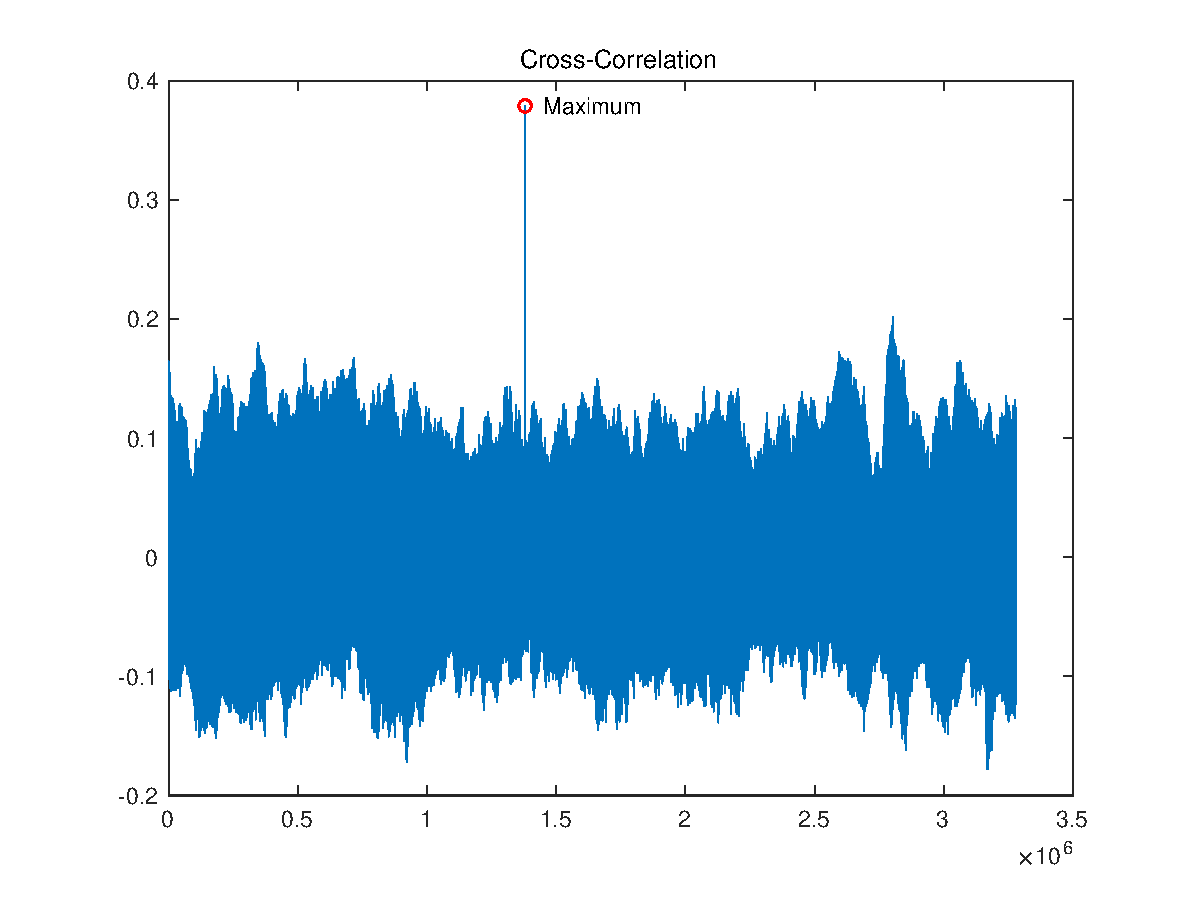
\includegraphics[width=0.40\linewidth]{figures/part1/crr_vis.eps}
	\end{center}
	\caption{Cross correlation 2D visualization}
	\label{fig:crr_vis}
\end{figure} 

\begin{figure}[h!]
	\begin{center}
		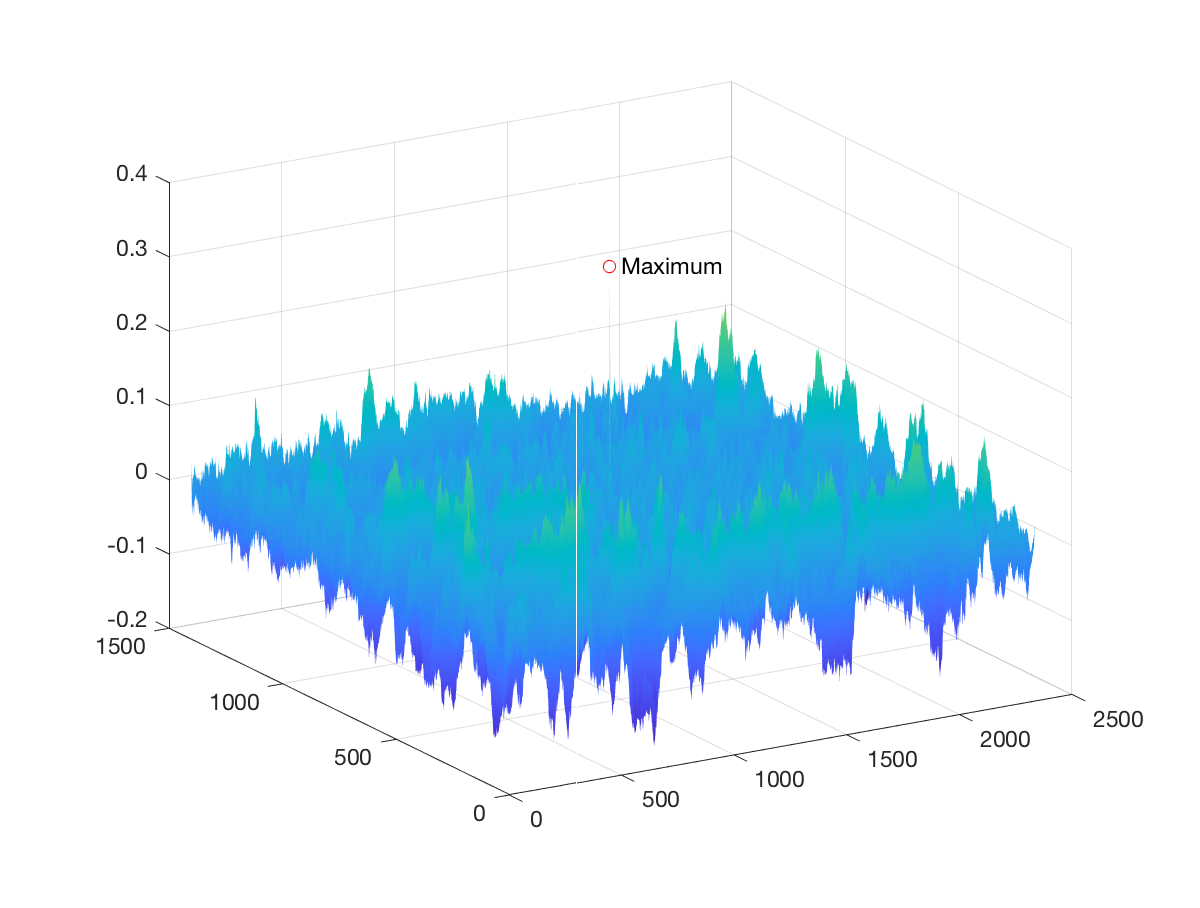
\includegraphics[width=0.40\linewidth]{figures/part1/crr_vis2.eps}
	\end{center}
	\caption{Cross correlation 3D visualization}
	\label{fig:crr_vis2}
\end{figure} 

\begin{figure}[h!]
	\centering
	\includegraphics[width=0.60\linewidth]{figures/part1/wallypuzzle_result.png}
\centering
\caption{Align result. }
\label{fig:maze-b}
\end{figure} 

\section{Spectral Cross Correlation}

Cross correlation can also be done in the spectral domain by completing a Fourier transform, multiplying signals, and doing an inverse Fourier transform.


\section{Pattern Finder}

